%class
	\documentclass{beamer}

%template
	\usetheme{HannoverSalman}
	\setbeamertemplate{navigation symbols}{}
	%\setbeamertemplate{footline}{\centering{\insertframenumber/\insertpresentationendpage}}
	%\setbeamertemplate{footline}{\hspace*{.5cm}\scriptsize{\hfill\insertframenumber\hspace*{.5cm}}} 


%packages
	\usepackage{amsmath, amssymb, graphicx,cancel}
	\usepackage[absolute,overlay]{textpos}
	\usepackage{subfigure}
	\usepackage{caption}\captionsetup{labelformat=empty,labelsep=none}
	\usepackage{geometry}
	\geometry{verbose}
	\usepackage{color}
	\usepackage{xmpmulti}
	\usepackage[3D]{movie15}
	\usepackage{hyperref}
%	\usepackage{bookmark}
	\usepackage[open,openlevel=4,atend]{bookmark}
	%\bookmarksetup{color=blue}
	\usepackage{multirow}
	\usepackage[style=numeric,defernumbers, authoryear]{biblatex}
	%\usepackage[square,sort]{natbib}
	%\usepackage{fancyhdr}%\pagestyle{fancy} 

	
	\hypersetup{bookmarksdepth = 4}


%citations files
	\bibliography{MyCitations}

%logoCSIPCPL
    \setlength{\TPHorizModule}{1mm}
    \setlength{\TPVertModule}{1mm}
    \newcommand{\logoCSIPCPL}
    {
    	\begin{textblock}{1}(100,2) %(100,85)  for bottom
    		
\includegraphics[width=1.5cm]{figs/logo_CSIP}
    	\end{textblock}
    	
	\begin{textblock}{1}(117,1) %(117,85)  for bottom
    		
\includegraphics[width=1.0cm]{figs/logo_CPL}
    	\end{textblock} 
    }

%logo evolution
    \newcommand{\logoEvolution}
    {    	
	\begin{textblock}{1}(110,1) %(117,85)  for bottom
    		\includegraphics[width=0.65in]{figs/logo_evolution.pdf}
    	\end{textblock} 
    }

%logo Qualcomm
    \newcommand{\logoQualcomm}
    {
    	\begin{textblock}{1}(110,2) %(100,85)  for bottom
    		\includegraphics[width=1.5cm]{figs/logo_qualcomm.jpg}
    	\end{textblock}
    }
%logo Qualcomm (long)
    \newcommand{\logoQualcommllong}
    {
    	\begin{textblock}{1}(0,0) 
    		\includegraphics[width=1.25in]{figs/logo_qualcomm_long.jpg}
    	\end{textblock}
    }

%logo Tech Tower
    \newcommand{\logoTechTower}
    {
    	\begin{textblock}{1}(0,0) 
    		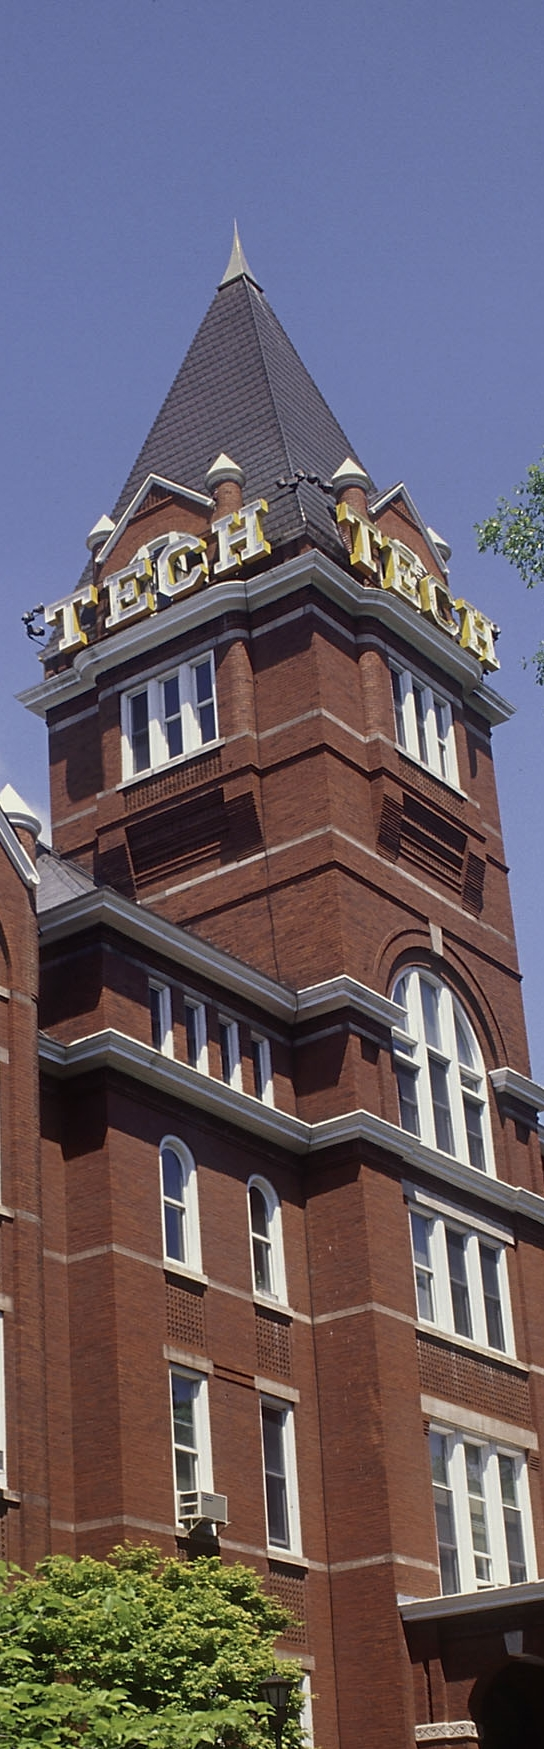
\includegraphics[width=1.25in]{figs/logo_TechTower.jpg}
    	\end{textblock}
    }

%logo tree
    \newcommand{\logoTree}
    {
    	\begin{textblock}{1}(0,0) 
    		\includegraphics[width=1.25in]{figs/logo_tree.jpg}
    	\end{textblock}
    }
%page numbers
    \newcommand{\mypagenum}
    {
    	\begin{textblock}{1}(1,94) 
		{\tiny \color[rgb]{0.2,0.2,1}\insertframenumber} %\insertframenumber,\insertpresentationendpage, \inserttotalframenumber
    	\end{textblock}
    }
%my footnote citation
	\newcommand{\myFootnoteCitation}[2]
	{
		\footnote{\tiny \citeauthor{#1}, \emph{#2}, \citeyear{#1}.}  %\citeauthor{#1}, \citetitle{#1}, #2 \citeyear{#1}.
	}
%my refer to citation
	\newcommand{\mycite}[1]
	{
		\emph{\citeauthor{#1} (\citeyear{#1})}
	}
%my footnote website citation
	\newcommand{\myFootnoteWebsiteCitation}[1]
	{
		\footnote{\tiny \citeauthor{#1}}
	}

\let\thefootnote\relax\footnotetext{Footnotetext without footnote mark}


%section underline
%\newcommand{\tmpsection}[1]{}
%\let\tmpsection=\section
%\renewcommand{\section}[1]{\tmpsection{\underline{#1}}}



%commands
	\newcommand{\likelihood}{p(Z_k| x_k) }						%likelihood
	\newcommand{\prior}{p(x_k)  } 								%prior
	\newcommand{\posterior} {p(x_k| Z_k)}						%posterior
	\newcommand{\prediction} {p(x_k| Z_{k-1})}					%prediction
	\newcommand{\update} {p(x_k|Z_k)}							%update
	\newcommand{\observations} {p(Z_k)}						%observations
	\newcommand{\prevobservations} {p(Z_{k-1})}				%previous observations
	\newcommand{\dxpk} {dx_{k-1}}							%dx_{k-1}
	\newcommand{\ChapKolm}{\int{p(x_k| x_{k-1})p(x_{k-1}|Z_{k-1})} \dxpk} %Chapman Kolmogorov

	%algorithm specific: JPDAF
	\newcommand{\likelihoodJPDAF}{p(Z_k| \chi, m, Z_{k-1}) }		%1. likelihood
	\newcommand{\priorJPDAF}{p(\chi|m, Z^{k-1}} 				%2. prior	
	\newcommand{\observationsJPDAF} {p(Z_k}					%3. observations
	\newcommand{\posteriorJPDAF} {p(\chi| Z_k)}					%4. posterior

%environments
	\newenvironment{changemargin}[2]
	{
	  	\begin{list}{}
		{
			\setlength{\topsep}{0pt}%
			\setlength{\leftmargin}{#1}%
			\setlength{\rightmargin}{#2}%
			\setlength{\listparindent}{\parindent}%
			\setlength{\itemindent}{\parindent}%
			\setlength{\parsep}{\parskip}%
		}
	  	\item[]
		}
		{\end{list}
	}
%figures

%colors
\definecolor{darkgreen}{rgb}{0,0.5,0}

%personal details
	\author{Salman Aslam}
	\institute{Advisor, Dr Christopher Barnes (ECE)\\Co-advisor, Dr Aaron Bobick (CoC)\\Georgia Institute of Technology}
	\date{}

\begin{document}
%####################################################################################################
\title{Pattern Recognition \\ and \\ Machine Learning}
%####################################################################################################
\begin{frame}\logoTree
	\institute{}
	\titlepage
\end{frame}

\begin{frame}\frametitle{Outline}\logoTree
	\setcounter{tocdepth}{1}	
	\tableofcontents
\end{frame}

%######################################################################
\section{INTRODUCTION}
%######################################################################
\begin{frame}
\frametitle{Introduction}
\frametitle{notation}
\logoCSIPCPL\mypagenum
	\begin{itemize}
		\item x: input (vector)
		\item $\theta$: parameter (vector)
		\item y: observation (vector)
		\item E: total error (scalar)
		\item J: energy (scalar)
	\end{itemize}
\end{frame}




\begin{frame}
\frametitle{Introduction}
\frametitle{problem statement}
\logoCSIPCPL\mypagenum
	\begin{itemize}
		\item Given:
			\begin{itemize}
				\item set of $N$ inputs, $x_0, x_1 \ldots x_{N-1}$
				\item set of $N$ outputs, $y_0, y_1 \ldots y_{N-1}$
			\end{itemize}
		\item Goal
			\begin{itemize}
				\item reproduce those outputs, $\hat{y}_0, \hat{y}_1 \ldots \hat{y}_{N-1}$
			\end{itemize}
	\end{itemize}
\end{frame}


\begin{frame}
\frametitle{Introduction}
\framesubtitle{inference}
\logoCSIPCPL\mypagenum
	There are 3 ways of doing inference:	
	\begin{itemize}
		\item Generative models
		\item Discriminative models
		\item Discriminant functions
	\end{itemize}
\end{frame}




\begin{frame}
\frametitle{Introduction}
\framesubtitle{inference: generative models}
\logoCSIPCPL\mypagenum
	\begin{itemize}
		\item Take training data and construct class conditional densities, $p(x|C_i)$
		\item Construct a model of the data for every class
		\item So, essentially, this is training
		\item For Gaussian class conditional densities,
			\begin{equation*}\tiny
			p(x|C_i) = \frac{1}{(2\pi)^{N/2}|\Sigma|^{1/2}}\text{exp}\left\{\frac{1}{2}(x-\mu)^T\Sigma^{-1}(x-\mu) \right\}
			\end{equation*}
		\item If there are 2 classes, then the priors are,
			\begin{align*}
				p(C_1)&=\pi   \\
				p(C_2)&=1-\pi 
			\end{align*}
	\end{itemize}
\end{frame}

%============================================================
\subsection{\ \ \ \ Statistical Learning Theory}
%============================================================

\begin{frame}[allowframebreaks]
In pattern recognition, the goal is to guess or predict the unknown nature of an observation, which is a $d$-dimensional collection of numerical measurements.  The goal is to create a function $g(x): R^d \rightarrow {1, 2, \ldots ,M}$, a mapping, a \emph{classifier} which errs on $x$ if $g(x) \neq y$.  A probabilistic setting is introduced where $(X,Y)$ is an $R^d$ x $\{1, 2, \ldots, M\}$-valued random pair.  The probability of error, the $loss$,  for classifier $g$ is $L(g) = \mathbf{P}(g(X) \neq Y)$.  If $\mathbf{P}(X,Y)$ is known,  the best possible classifier, the \emph{Bayes classifier} $g^*$ can be computed as arg $\min\limits_{g:R^d \rightarrow {1, 2, \ldots, M}} \mathbf{P}(g(X) \neq Y)$ with corresponding minimum loss $L^* = L(g^*)$.  Since $\mathbf{P}(X,Y)$ is in general not known, an assumption is made that a sequence of independent identically distributed (i.i.d.) data with the same distribution as that of $\mathbf{P}(X,Y)$ is given.
\end{frame}

\begin{frame}
\frametitle{Introduction}
\framesubtitle{SLT: history}
\logoCSIPCPL\mypagenum
History of statistical learning, leading up to SVMs:
	\begin{itemize}
		\item Statistical inference started with Gauss and Laplace more than 200 years ago.
		\item Till about the late 1920s, descriptive statistics was mostly complete.
		\item Systematic analysis of statistical inference started in the late 1920s.
		\item The question to be investigated now was finding a reliable method of statistical inference.  Two main ideas emerged:
			\begin{enumerate}
				\item Parametric Statistical Inference
				\item General Statistical Inference
			\end{enumerate}
	\end{itemize}
\end{frame}  



\begin{frame}
\frametitle{Introduction}
\framesubtitle{SLT history: parametric statistical inference}
\logoCSIPCPL\mypagenum
	\begin{itemize}
		\item Fisher worked in parametric statistics and introduced the ML method.  
		\item This parametric method aims to create simple statistical models of inference that can be used for solving real life problems.  
		\item Here, the investigator knows the problem to be analyzed quite well.  
		\item Shortcomings in this approach started to be felt when computers could work with larger datasets, i.e. the curse of dimensionality.  Statisticians turned to more general methods.
	\end{itemize}
\end{frame}


\begin{frame}
\frametitle{Introduction}
\framesubtitle{SLT history: general statistical inference}
\logoCSIPCPL\mypagenum
	\begin{itemize}
		\item Glivenko, Cantelli and Kolmogorov started a general analysis of statistical inference.  
		\item Here, one does not have reliable a priori information about the statistical law underlying the problem.  
		\item It is necessary to find a method to infer an approximating function from the given examples.  
		\item The results of Glivenko, Cantelli and Kolmogorov started more than 40 years of research that culminated in inductive methods.   
		\item It started with Rosenblatt's perceptron, leading to the Empirical Risk Minimization (ERM) principle on indicator functions (i.e. pattern recognition) and then on real valued functions (i.e. regressions, density estimations, etc.).  
	\end{itemize}
\end{frame}



\begin{frame}
\frametitle{Introduction}
\framesubtitle{SLT history: general statistical inference (cont.)}
\logoCSIPCPL\mypagenum
	\begin{itemize}
		\item Vapnik and Chervonenkis showed that consistency and the rate of convergence of the ERM principle is related to the VC dimension, 
			\begin{itemize}
				\item i.e. for distribution independent consistency of the ERM principle, it is necessary and sufficient that the set of functions implemented by the learning machine has a finite VC dimension.  
			\end{itemize}
		\item To achieve smallest bound on test errors, a learning machine with smallest VC dimension must be used.  
		\item But to minimize number of training errors, a learning machine with high VC dimension must be used.  
		\item To find best guaranteed solution, a compromise is needed, and this is formalized in the induction principle of Structured Risk Minimization (SRM), which eventually led to the discovery of SVMs.
	\end{itemize}
\end{frame}


\begin{frame}
\frametitle{Introduction}
\framesubtitle{SLT: theories of learning}
\footnote{John Shawe Taylor}
\logoCSIPCPL\mypagenum
	\begin{itemize}
		\item SLT (statistical learning theory)
		\item Bayesian inference
		\item Inductive inference
		\item Statistical physics
		\item Traditional statistical analysis
	\end{itemize}
\end{frame}


\begin{frame}
\frametitle{Introduction}
\framesubtitle{SLT: general statistical considerations}
\footnote{John Shawe Taylor}
\logoCSIPCPL\mypagenum
	\begin{enumerate}
		\item Statistical models (not including Bayesian) have very little knowledge of how data is generated
			\begin{itemize}
				\item data is generated by a distribution $P$ typically not known
				\item instead, we have a "training sample" or training set
					\begin{equation*}
						\mathcal{S} = {(x_1, y_1), \ldots (x_m, y_m)}
					\end{equation*}
			\end{itemize}
		\item $S$ generated independently and identically from $P$
	\end{enumerate}
\end{frame}


\begin{frame}
\frametitle{Introduction}
\framesubtitle{SLT: notation}
\logoCSIPCPL\mypagenum
	\begin{itemize}
		\item Notation
			\begin{enumerate}
				\item {\color{red}$\mathcal{A}$}: learning algorithm 
				\item {\color{red}$\mathcal{F}$}: function class
				\item {\color{red}$\mathcal{A}$}: training set
				\item {\color{red}$\mathcal{A_\mathcal{F}(\mathcal{S})}$}: function chosen by $\mathcal{A}$ from $\mathcal{F}$ in response to $\mathcal{S}$
					\begin{itemize}
						\item actual choice of function depends on $\mathcal{S}$
						\item different $\mathcal{S}$ for same $\mathcal{A}$ will result in a different function, hopefully not too different
					\end{itemize}
				\item {\color{red}$\mathcal{A_\mathcal{F}(\mathcal{S})}(x)$}: $\mathcal{A_\mathcal{F}(\mathcal{S})}$ applied to test example $(x, y)$
				\item {\color{red}$l$}: loss, discrepancy between $\mathcal{A_\mathcal{F}(\mathcal{S})}(x)$ and $y$
				\item {\color{red}$\epsilon(\mathcal{S,A,F})$}: expected value of loss, $\mathbb{E}[l] =  \mathbb{E}[l(\mathcal{A_\mathcal{F}(\mathcal{S})}, x, y)]$
			\end{enumerate}
		\begin{equation*} 
			\epsilon
		\end{equation*}
	\end{itemize}
\end{frame}


%============================================================
\subsection{\ \ \ \ Dempster Schafer}
%============================================================
\begin{frame}
\frametitle{Introduction}
\framesubtitle{Dempster Schafer}
\logoCSIPCPL\mypagenum
	\begin{figure}				
		\includegraphics[height=0.8\textheight]{figs/PRML_Dempster_Schafer_cat_example.pdf}
	\end{figure}
\end{frame}


%============================================================
\subsection{\ \ \ \ PCA}
%============================================================

\begin{frame}
\frametitle{Introduction}
\framesubtitle{PCA: overview}
\logoCSIPCPL\mypagenum
	{\color{red}Goal:} Rotate basis so that it better explains input data	\\
	\begin{figure}
		\includegraphics[width=1.0\textwidth]{figs/PRML_PCA_blockDiagram.pdf}
	\end{figure}
\end{frame}


\begin{frame}
\frametitle{Introduction}
\framesubtitle{PCA: derivation (overview)}
\logoCSIPCPL\mypagenum
	modern reference: Jolliffe, 2002\\
	\vspace{0.1in}
	{\color{red}Geometric derivation steps (Pearson, 1901):} 
	\begin{enumerate}
		\item {\color{blue} Compute total projection error}
		\item {\color{blue} Find expression for projection magnitude}
		\item {\color{blue} Maximize projection magnitude, i.e. minimize projection error}
	\end{enumerate}
	\vspace{0.1in}
	{\color{red}Algebraic derivation steps (Hotelling, 1933):} 
	\begin{enumerate}
		\item {\color{blue} Project data:} Take an arbitrary unit vector $q$, and project our data on this vector, $y = q^Tx$
		\item {\color{blue} Find variance of projected data:}  $\sigma^2(y)$
		\item {\color{blue} Maximize variance:} Move $q$ so that it maximizes the variance of this  projected data, $\sigma^2(y)$
	\end{enumerate}
\end{frame}


\begin{frame}
\frametitle{Introduction}
\framesubtitle{PCA: algebraic derivation, step 1: project data}
\logoCSIPCPL\mypagenum
	\begin{itemize}
		\item Pick arbitrary $q$ %The goal is to align it with direction of maximum data spread
		\item Find projected data $y=q^Tx$
	\end{itemize}	
	\begin{figure}
		\includegraphics[width=0.8\textwidth]{figs/PRML_PCA_IITkharagpur_1.pdf}
	\end{figure}
\end{frame}



\begin{frame}
\frametitle{Introduction}
\framesubtitle{PCA: algebraic derivation, step 2: find variance of projected data}
\logoCSIPCPL\mypagenum
	\begin{itemize}
 		\item The variance of $y$ is given by,
			\begin{align*}
			 \sigma^2_y(q) &= E[y^2]\\
				&= E[q^Txx^Tq] \\
				&= q^TRq	
			\end{align*}
 		\item Here $R$ is the correlation matrix of $x$
		\item We write $\sigma^2_y(q)$ and not simply $\sigma^2_y$ since the variance of $y$ depends on the choice of $q$  	
		\item We want maximum variance
		\item As a sidenote, the mean of $y, E[y] = E[q^Tx]=0$
	\end{itemize}
\end{frame}			



\begin{frame}
\frametitle{Introduction}
\framesubtitle{PCA: algebraic derivation, step 3: maximize variance of projected data}
\logoCSIPCPL\mypagenum
	\begin{figure}
		\includegraphics[height=0.8\textheight]{figs/PRML_PCA_IITkharagpur_2.pdf}
	\end{figure}
\end{frame}


\begin{frame}[plain]
\frametitle{Introduction}
\framesubtitle{PCA: geometric derivation, notation}
\logoCSIPCPL\mypagenum
	\begin{changemargin}{-1.3in}{0in} 
		\begin{figure}
			\includegraphics[width=1.35\textwidth]{figs/PRML_PCA_geometricDerivation_notation.pdf}
		\end{figure}
	\end{changemargin}
\end{frame}


\begin{frame}
\frametitle{Introduction}
\framesubtitle{PCA: geometric derivation, step 1: compute total projection error}
\logoCSIPCPL\mypagenum	
	\begin{figure}
		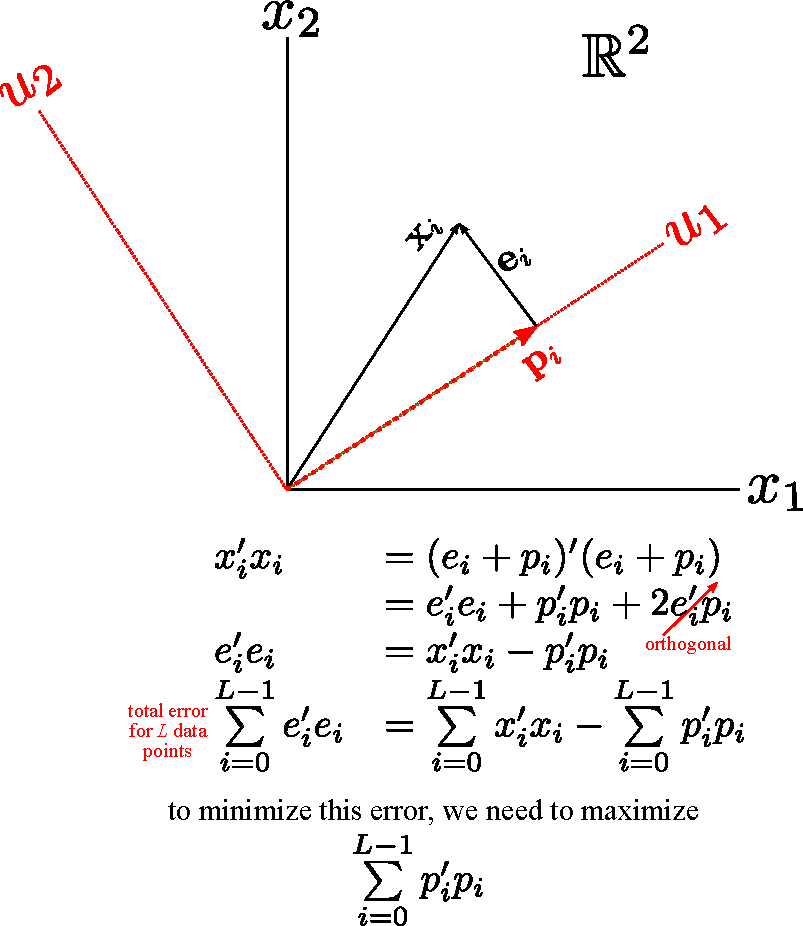
\includegraphics[height=0.85\textheight]{figs/PRML_PCA_geometricDerivation_step1.pdf}
	\end{figure}
\end{frame}



\begin{frame}
\frametitle{Introduction}
\framesubtitle{PCA: geometric derivation, step 2: find expression for projection magnitude}
\logoCSIPCPL\mypagenum	
	\begin{figure}
		\includegraphics[width=1.0\textwidth]{figs/PRML_PCA_geometricDerivation_step2.pdf}
	\end{figure}
	\begin{itemize}
		\item in the next slide, we begin with $B'\Sigma B$ instead of $V_q'\Sigma Vq$
		\item we show that this quantity is maximized when $B=V_q$
		\item maximizing $B'\Sigma B$, i.e. setting it equal to $V_q'\Sigma Vq$ minimizes projection error
	\end{itemize}
\end{frame}



\begin{frame}[plain]
\frametitle{Introduction}
\framesubtitle{PCA: geometric derivation, step 3: maximize projection magnitude, i.e. minimize projection error}
\logoCSIPCPL\mypagenum
	\begin{changemargin}{-1.3in}{0in}	
		\begin{figure}
			\includegraphics[width=1.35\textwidth]{figs/PRML_PCA_geometricDerivation_step3.pdf}
		\end{figure}
	\end{changemargin}
\end{frame}


\begin{frame}
\frametitle{Introduction}
\framesubtitle{PCA: Dimensionality reduction}
\logoCSIPCPL\mypagenum
	\begin{itemize}
		\item project each data point onto new axes
		\item some of the projections will be very small, and can be ignored
		\item each data point can therefore be represented by fewer dimensions
		\item for each data point, the relevant dimensions will be different
	\end{itemize}
\end{frame}



\begin{frame}
\frametitle{Introduction}
\framesubtitle{PCA: vs K-means}
\framesubtitle{}
\logoCSIPCPL\mypagenum
\myFootnoteCitation{2004_CNF_KmeansVsPCA_DingHe}{ICML}
	\begin{figure}
		\includegraphics[width=0.7\textwidth]{figs/SP_covariance_detailed.pdf}
	\end{figure}
\end{frame}


%=======================================
\subsection{\ \ \ \ wavelets}
%=======================================
\begin{frame}
\frametitle{Introduction}
\framesubtitle{wavelets}
\logoCSIPCPL\mypagenum
	\begin{figure}				
		\includegraphics[width=1.0\textwidth]{figs/MT_wavelets.pdf}
	\end{figure}
\end{frame}

\begin{frame}
\frametitle{Introduction}
\framesubtitle{Haar wavelets}
\logoCSIPCPL\mypagenum
	\begin{figure}				
		\includegraphics[height=0.8\textheight]{figs/MT_wavelets_Haar.pdf}
	\end{figure}
\end{frame}


%=======================================
\subsection{\ \ \ \ SVM}
%=======================================
\begin{frame}
\frametitle{Introduction}
\framesubtitle{SVM}
\logoCSIPCPL\mypagenum
	\begin{itemize}
		\item One kind of kernel technique, 
		\item Easy to use
		\item Define an indicator vector $y$
		\item Feature vectors in Euclidean space, like width, height
		\item Every vector is a data instance 
		\item $y_i=1$ if $x_i$ in class 1
		\item $y_i=-1$ if $x_i$ in class 2
		\item Find a separating hyperplane
			\begin{equation*}
				w^tx + b=0
			\end{equation*}
		\item Decision function, $f(x)=sgn(w^tx + b)$
		\item Many possible choices of $w$ and $b$
		\item If data is not linearly separable the optimization becomes infeasible, so you allow training errors
	\end{itemize}
\end{frame}




\begin{frame}
\frametitle{Introduction}
\framesubtitle{SVM: linear discriminant function}
\logoCSIPCPL\mypagenum
	\begin{figure}				
		\includegraphics[height=0.8\textheight]{figs/PRML_discriminantFunction.pdf}
	\end{figure}
\end{frame}



\begin{frame}
\frametitle{Introduction}
\framesubtitle{SVM: Matlab packages}
\logoCSIPCPL\mypagenum
	\tiny
	These 6 are given on the following pages:
{\color{blue}  \href{http://www.cs.ubc.ca/~murphyk/Software/svm.htm}{http://www.cs.ubc.ca/\textasciitilde murphyk/Software/svm.htm}} and
{\color{blue}  \href{http://www.svms.org/software.html}{http://www.svms.org/software.html}}
	\tiny
	\begin{enumerate}
		\item LearnSC (no source)\\ 
{\color{blue} \href{http://www.support-vector.ws/html/downloads.html}
{http://www.support-vector.ws/html/downloads.html }}
		\item LibSVM \\
{\color{blue}  \href{http://www.csie.ntu.edu.tw/~cjlin/libsvm/}{http://www.csie.ntu.edu.tw/~cjlin/libsvm/}}
		\item LS-SVM\\
{\color{blue}\href{http://www.esat.kuleuven.ac.be/sista/lssvmlab/ }
{http://www.esat.kuleuven.ac.be/sista/lssvmlab/ }}
		\item Matlab SVM toolbox \\ 
{\color{blue} \href{http://www.isis.ecs.soton.ac.uk/resources/svminfo/}{http://www.isis.ecs.soton.ac.uk/resources/svminfo/}}
		\item OSU SVM (old)\\
{\color{blue} \href{http://sourceforge.net/projects/svm/}
{http://sourceforge.net/projects/svm/}}
		\item Spider (old)\\ 
{\color{blue} \href{http://www.kyb.tuebingen.mpg.de/bs/people/spider/}{http://www.kyb.tuebingen.mpg.de/bs/people/spider/}}
	\end{enumerate}
	additional:
	\tiny
	\begin{enumerate}
	\item LSVM, ASVM and PSVM\\
{\color{blue} \href{http://www.cs.wisc.edu/dmi/lsvm/}
{http://www.cs.wisc.edu/dmi/lsvm/}}\\
{\color{blue} \href{http://www.cs.wisc.edu/dmi/asvm/}
{http://www.cs.wisc.edu/dmi/asvm/}}\\
{\color{blue} \href{http://www.cs.wisc.edu/dmi/psvm/}
{http://www.cs.wisc.edu/dmi/psvm/}}
	\item SVM and kernel methods toolbox\\
{\color{blue} \href{http://asi.insa-rouen.fr/enseignants/~arakotom/toolbox/index.html}
{http://asi.insa-rouen.fr/enseignants/~arakotom/toolbox/index.html}}\\
	\end{enumerate}
\end{frame}

%######################################################################
\subsection{\ \ \ \ kernel methods}
%######################################################################
\begin{frame}
\frametitle{Introduction}
\framesubtitle{kernel methods: similarity and learning \footnote{Brian Sch\"{o}lkopf}}
\logoCSIPCPL\mypagenum
	\begin{itemize}
		\item input/output sets $\mathcal{X, Y}$
		\item training set $(x_1, y_1), \ldots (x_L, y_L) \in \mathcal{X} \mbox{x} \mathcal{Y}$
		\item {\color{red}generalization}: given a previously unseen $x \in \mathcal{X}$, find a suitable $y \in mathcal{Y}$
		\item $(x,y)$ should be {\color{red}"similar"} to $(x_1, y_1), \ldots (x_L, y_L)$
		\item how to measure similarity?
			\begin{itemize}
				\item for outputs: {\color{red}loss function}, e.g. zero-one loss for $\mathcal{Y} = \{\pm 1\}$
				\item for inputs: {\color{red}kernel}
			\end{itemize}
	\end{itemize}
\end{frame}



\begin{frame}
\frametitle{Introduction}
\framesubtitle{kernel methods: similarity of inputs (kernels)\footnote{Brian Sch\"{o}lkopf}}
\logoCSIPCPL\mypagenum
	\begin{enumerate}
		\item {\color{red}function} 
			\begin{itemize}
				\item symmetric function, $k: \mathcal{X}\mbox{x}\mathcal{Y} \rightarrow \mathbb{R}$
				\end{itemize}
		\item {\color{red}inputs} 
			\begin{itemize}
				\item take 2 inputs $x$ and $x'$
				\item say one face and one non-face, or 
				\item both faces, or 
				\item both non-faces, and 
				\item assign a kernel value to this pair, $(x,x') \mapsto k(x,x')$
			\end{itemize}
		\item {\color{red}output}  
			\begin{itemize}
				\item {\color{blue} if $\mathcal{X}$ is a vector space},
					\begin{itemize}
						\item $\mathcal{X} = \mathbb{R}^N$
						\item one possible kernel is the canonical dot product, $k(x,x') = \sum_{i=1}^N x_i x'_i$
					\end{itemize}
				\item {\color{blue} if $\mathcal{X}$ is not a dot product space}, 
					\begin{itemize}
						\item we assume that $k$ is a dot product in a linear space $\mathcal{H}$, 
						\item i.e. there exists a map $\Phi: \mathcal{X} \mapsto \mathcal{H}$ such that $k(x,x') = \langle \Phi(x), \Phi(x') \rangle$
						\item we can have geometric algorithms in the dot product space (feature space), $\mathcal{H}$
					\end{itemize}
			\end{itemize}
	\end{enumerate}
\end{frame}




\begin{frame}
\frametitle{Introduction}
\framesubtitle{kernel methods}
\logoCSIPCPL\mypagenum
	\begin{itemize}
		\item We have $n$ observations in euclidean $R^D$ drawn from unknown distribution $p(x)$
		\item {\color{red}Goal: } Estimate $p(x)$
	\end{itemize}
\end{frame}




\begin{frame}
\frametitle{Introduction}
\framesubtitle{kernel methods: notation}
\logoCSIPCPL\mypagenum
	\begin{itemize}
		\item {\color{red}$N$}: number of data points
		\item {\color{red}$D$}: number of dimensions
	 	\item {\color{red}$p(x)$}: distribution of {\color{red}$x$}
		\item {\color{red}$R$}: small region containing {\color{red}$K$} data points (a subset of all the data points in $x$)
		\item {\color{red}$V$}: volume of $R$
		\item {\color{red}$P$}: each point in $x$ has probability $P$ of falling in $R$, where
			\begin{equation*}
				P=\int_R p(x)dx
			\end{equation*}
		\item {\color{red}\text{bin}$(K|N,P)$}: binomial distribution for $K$
		\item {\color{red} $k(u)$}: unit square centered on origin, a Parzen window
			\begin{equation*}
				k(u) = 
				\left\{ 
				\begin{array}{rl}
					1\text{,} &  |u_i|<1/2 \ \ \ \ \ \ \ \ \ i=1,\ldots, D\\ 
					0\text{,} &  \mbox{otherwise}
				\end{array}
				\right.
			\end{equation*}
	\end{itemize}
\end{frame}


\begin{frame}
\frametitle{Introduction}
\framesubtitle{kernel density, step 1: find $K$}
\logoCSIPCPL\mypagenum
	\begin{itemize}
 		\item $K$ is distributed as,
			\begin{equation*}
				p(K) = \text{bin}(K|N,P) =
				\left(
					\begin{array}{c}
						 N \\ K	
					\end{array}
				\right)
				P^K(1-P)^{N-K}
			\end{equation*}
			\item notice the usage of $P$ rather than $p$
				\begin{itemize}
					\item this is because a success is measured if a point lies in $R$, and the probability for that is $P$, not $p$
				\end{itemize}
		\item E$[K] = NP$ (from binomial distribution)
		\begin{itemize}
			\item for large $N$, $K \simeq NP$
			\item for small $V$, $P=p(x)V$ 
				\begin{block}{}
					\begin{align*} 
						K &\simeq Np(x)V\\
						&= Np(x)h^D \ \ \ \text{(using volume of cube with length $h$)}
					\end{align*}
				\end{block}
			\item large $n$ and small $V$ are contradictory requirements
			\item fix $k$, find $V$, {\color{red}nearest neighbor approach}
			\item fix $V$, find $K$, {\color{red}kernel approach}
		\end{itemize}
	\end{itemize}
\end{frame}



\begin{frame}
\frametitle{Introduction}
\framesubtitle{kernel density: step 2, find $K$ (different formulation)}
\logoCSIPCPL\mypagenum
	\begin{itemize}
		\item let's center a cube of length $h$ on $x$,
			\begin{equation*}
				k\left(\frac{x-x_n}{h}\right) = 
				\left\{ 
				\begin{array}{rl}
					1\text{,} &  x_n \ \mbox{inside cube}\\ 
					0\text{,} &  \mbox{otherwise}
				\end{array}
				\right.
			\end{equation*}
		\item therefore, total number of data points inside cube,
			\begin{block}{}
				\begin{equation*}
					K = \sum\limits_{i=1}^{N}k\left(\frac{x-x_n}{h}\right)
				\end{equation*}
			\end{block}
	\end{itemize}
\end{frame}


\begin{frame}
\frametitle{Introduction}
\framesubtitle{kernel density: step 3, equate $K$}
\logoCSIPCPL\mypagenum
	\begin{equation*} 
		Np(x)V = \sum\limits_{i=1}^{N}k\left(\frac{x-x_n}{h}\right)
	\end{equation*}
	\begin{block}{Parzen kernel density estimator}
		\begin{equation*}
			p(x) = \frac{1}{NV} \sum\limits_{i=1}^{N}k\left(\frac{x-x_i}{h}\right)
		\end{equation*}
	\end{block}
	Steps to compute kernel density at point $x$
	\begin{enumerate}
		\item Center a window on $x$
		\item Go through all data points and increment counter if they fall in this window
		\item Divide this number by $NV$
		\item This is the value of the density at that $x$
	\end{enumerate}
\end{frame}


\begin{frame}
\frametitle{Introduction}
\framesubtitle{Gaussian kernel}
\logoCSIPCPL\mypagenum
	\begin{equation*}
		p(x) = \frac{1}{N} \sum\limits_{i=1}^{N}\frac{1}{\sqrt{2\pi h^2}}e^{-\frac{\Vert x-x_n\Vert^2}{2 h^2}}
	\end{equation*}
	Kernel requirements
	\begin{align*}
		k(u) &\geq 0 \\
		\int k(u)du &= 1
	\end{align*}
\end{frame}


\begin{frame}
\frametitle{Introduction}
\framesubtitle{mean shift {\small (adaptive gradient ascent)}: derivation}
\logoCSIPCPL\mypagenum
	\begin{figure}				
		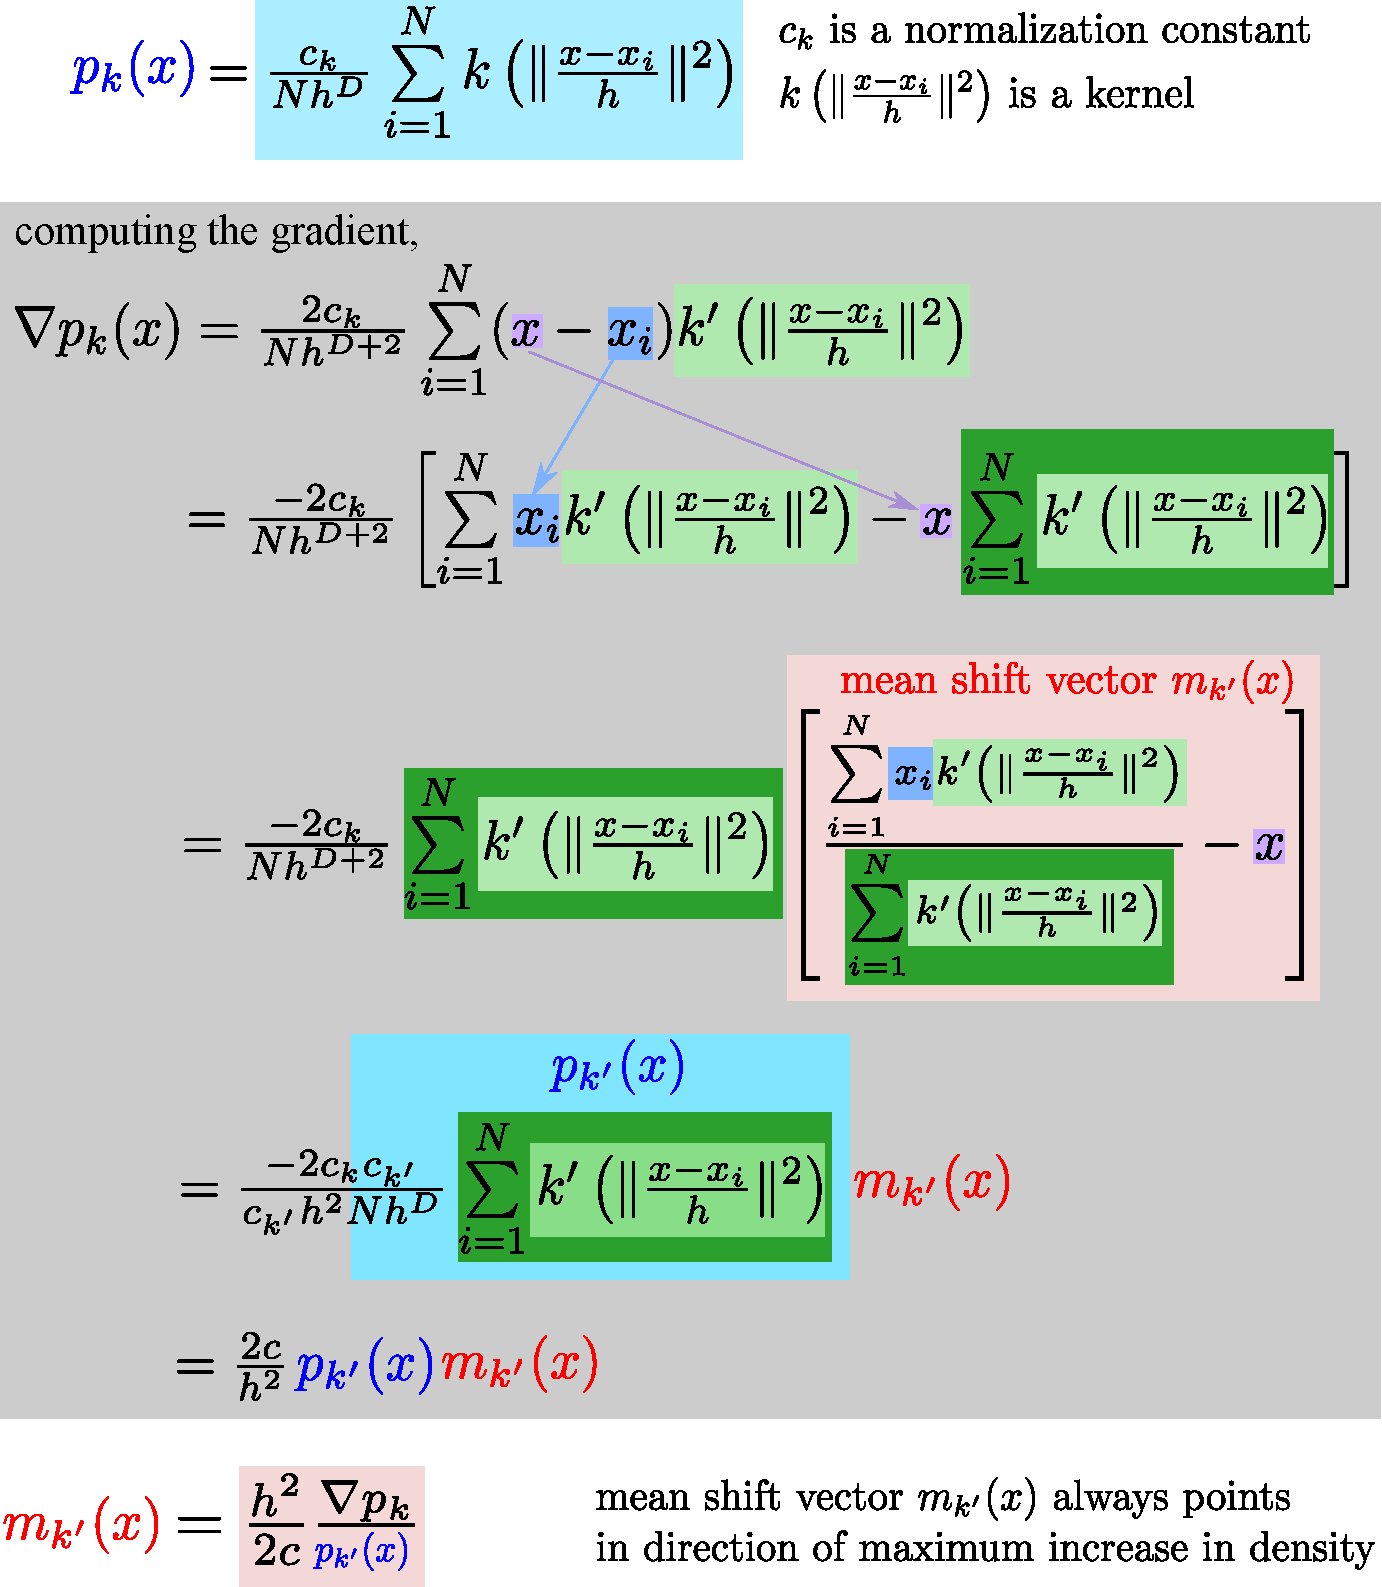
\includegraphics[height=.85\textheight]{figs/PRML_meanShift.pdf}
	\end{figure}
\end{frame}


\begin{frame}
\frametitle{Introduction}
\framesubtitle{mean shift {\small (adaptive gradient ascent)}: segmentation}
\logoCSIPCPL\mypagenum
	\begin{itemize}				
		\item For a pixel, compute its mean shift vector
		\item This mean shift vector ends at a mode of the density
		\item Repeat for all pixels, now you have a bunch of modes
		\item The set of all locations that converge to the same mode defines the  {\color{red}\emph {basin of attraction}} of that mode
		\item Merge (i.e. prune) modes that are close to each other, and corresponding basins of attraction
	\end{itemize}
\end{frame}




\begin{frame}
\frametitle{Introduction}
\framesubtitle{mean shift {\small (adaptive gradient ascent)}: segmentation}
\logoCSIPCPL\mypagenum
\myFootnoteCitation{2003_JNL_TRKkernel_Comaniciu}{PAMI}
	\begin{itemize}				
		\item 7 pruned nodes
		\item 7 corresponding basins of attraction (i.e. clusters, or segmented regions)
	\end{itemize}
	\begin{figure}
		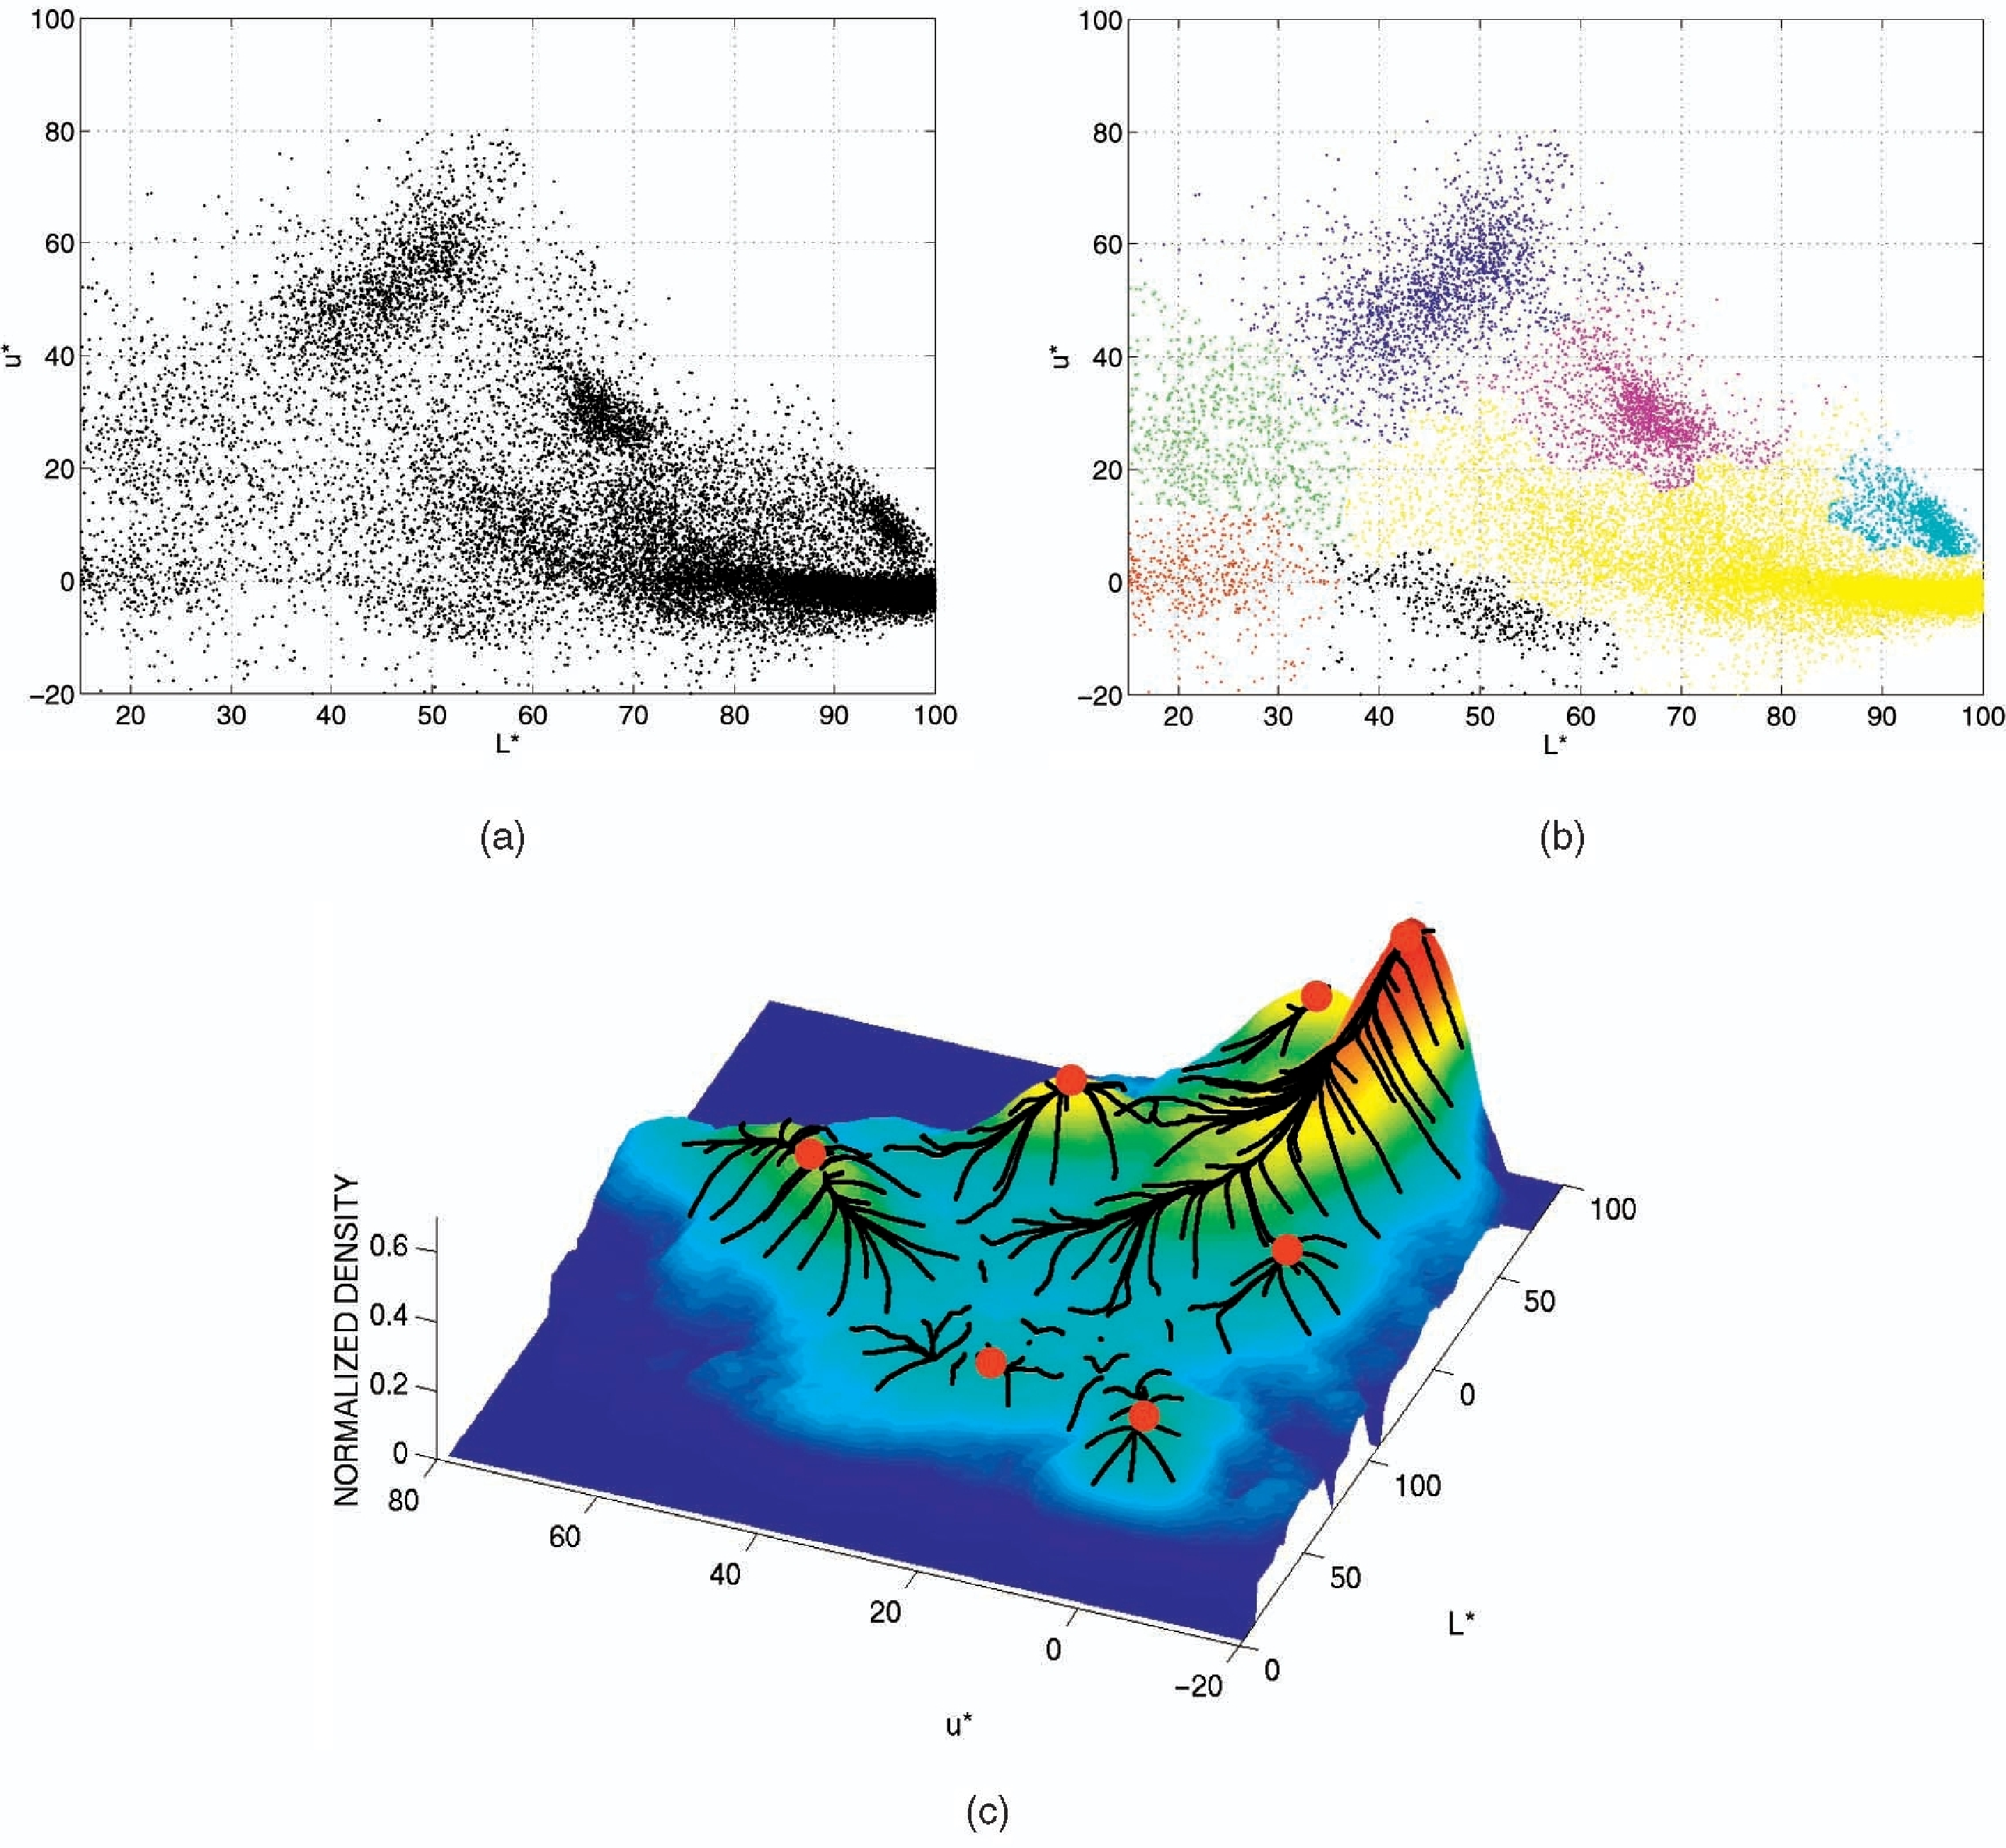
\includegraphics[height=0.6\textheight]{figs/PRML_meanShift2.pdf}
	\end{figure}
\end{frame}



%======================================
\subsection{\ \ \ \ Markov models}
%======================================
\begin{frame}
\frametitle{Introduction}
\framesubtitle{OMM}
\logoCSIPCPL\mypagenum
	{\color{red} OMM}\\
	Each state corresponds to an observable (physical) event
	\begin{figure}				
		\includegraphics[width=.50\textwidth]{figs/HMM_OMM_example.pdf}
	\end{figure}
\end{frame}




\begin{frame}
\frametitle{Introduction}
\framesubtitle{OMM}
\logoCSIPCPL\mypagenum
	\begin{align*}
		p(X_n) 	&= p(x_n| X_{n-1})p(X_{n-1})   	  						\\
				&= p(x_n| x_{n-1}) p(X_{n-1})   							\\  
				&= p(x_n| x_{n-1}) p(x_{n-1}| X_{n-2})p(X_{n-2})  			\\	
				&= p(x_n| x_{n-1}) p(x_{n-1}| x_{n-2}) ... p(x_2|x_1)p(x_1)  	
	\end{align*}
\end{frame}




\begin{frame}
\frametitle{Introduction}
\framesubtitle{OMM, example}
\logoCSIPCPL\mypagenum
	\begin{itemize}
		\item We study the probability of getting a set of 8 observations
		\item $O={S_3, S_3, S_3, S_1, S_1, S_3, S_2, S_3}$.  
		\item Given: Day 1, it is sunny ($S_3$)
		\item What is the probability that for the next 7 days, we will get sun-sun-rain-rain-sun-cloudy-sun?  	
	\end{itemize}
	\begin{align*}
		\tiny
		p(O&={S_3, S_3, S_3, S_1, S_1, S_3, S_2, S_3}) \\
		&= p(S_3)p(S_3|S_3)p(S_3|S_3)p(S_1|S_3)p(S_1|S_1)p(S_3|S_1)p(S_2|S_3)p(S_3|S_2) \\
		&=(1)(0.8)(0.8)(0.1)(0.4)(0.3)(0.1)(0.2)  \\
		&=1.536*10^{-4} 
	\end{align*}
\end{frame}	




\begin{frame}
\frametitle{Introduction}
\framesubtitle{HMM}
\logoCSIPCPL\mypagenum
	\begin{itemize}
		\item {\color{red}Observable Markov Model (OMM)}
			\begin{itemize}
				\item each state corresponds to an observable (physical) event
				\item restrictive model
				\item extended so that each observation is a probabilistic function of the state
			\end{itemize}
		\item {\color{red}Hidden Markov Model (HMM)}
			\begin{itemize}
				\item Doubly embedded stochastic process
				\item Underlying stochastic process is not observable 
				\item Can only be observed through another  stochastic process
			\end{itemize}
	\end{itemize}
\end{frame}




\begin{frame}
\frametitle{Introduction}
\framesubtitle{HMM}
\logoCSIPCPL\mypagenum
	\begin{figure}				
		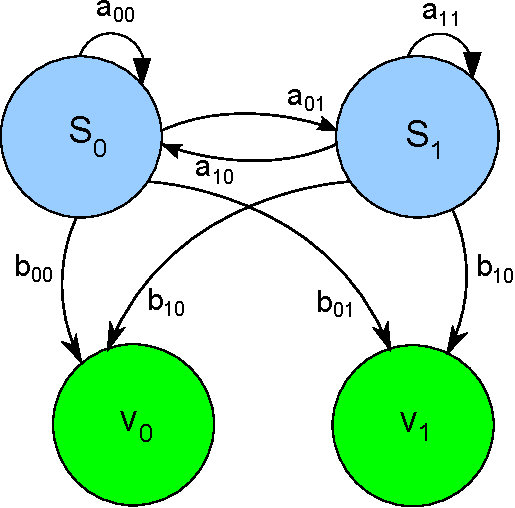
\includegraphics[width=.50\textwidth]{figs/HMM_flowDiagram.pdf}
		\caption{Hidden Markov Model}
	\end{figure}
\end{frame}




\begin{frame}
\frametitle{Introduction}
\framesubtitle{HMM}
\logoCSIPCPL\mypagenum
	\begin{enumerate}
		\item {\color{red} States, S} 
			\begin{itemize}
				\item $\{S_1, S_2, ... S_N\}$
				\item state at time $t$ is $q_t$
			\end{itemize}
		\item {\color{red} Observations/state, $V$}
			\begin{itemize}
				\item $\{v_1, v_2, ... v_M\}$
				\item Each observation $O_t$ is one of the symbols from $V$
				\item $T$ is the number of observations in the sequence
			\end{itemize}
		\item {\color{red} State transition probability distribution, A}  
			\begin{itemize}
				\item For the special case where every state can reach every other state, $a_{ij}>0$
					\begin{equation*}
						a_{ij} = p(q_{t+1}=S_j|q_t=S_i)  \ \ \ \ \ 1 \leq i, j \leq N
					\end{equation*}
			\end{itemize}
		\item {\color{red}Observation symbol probability distribution, B}
			\begin{equation*}
				b_{jk} = p(v_k|q_t=S_j)  \ \ \ \ \ 1 \leq j \leq N,  1 \leq k \leq M
			\end{equation*}
		\item {\color{red}Initial distribution}
			\begin{equation*}
				\pi_i	= P(q_1=S_i) \ \ \ \ \ 1 \leq i \leq N
			\end{equation*}
	\end{enumerate}
\end{frame}





\begin{frame}
\frametitle{Introduction}
\framesubtitle{HMM}
\logoCSIPCPL\mypagenum
	\begin{itemize}
		\item Complete parameter set of the model
				\begin{equation*}
					\lambda = (A, B, \pi)
				\end{equation*}
		\item Given appropriate values of $N, M, \lambda$
			\begin{itemize}
				\item Observation sequence $O_1, O_2, \ldots O_T$ can be generated
				\item Model for how a given observation was generated by an appropriate HMM
			\end{itemize}
	\end{itemize}
\end{frame}


\begin{frame}
\frametitle{Introduction}
\framesubtitle{HMM, 3 basic problems}
\logoCSIPCPL\mypagenum
	{\color{red}Testing}\\
	Given the observation sequence $O_1, O_2, ... O_T$, and a model $\lambda=(A, B, \pi)$, how do we compute	
	\vspace{0.1in}
	\begin{enumerate}	
		\item {\color{blue} Evaluation problem} $p(O|\lambda)$ Use of forward backward algorithm.
		\item  {\color{blue} Posterior} Use Viterbi algorithm
		\begin{equation*} 
			\max_{q_1, q_2, ... q_T}p(q_1, q_2, ... q_t, O_1, O_2, ... O_t|\lambda)
		\end{equation*}
	\end{enumerate}
	\vspace{0.3in}
	{\color{red}Training}\\
	How do we adjust the model parameters $\lambda=(A, B, \pi)$ to maximize $p(O|\lambda)$.
	\vspace{0.1in}
	\begin{enumerate}\setcounter{enumi}{2}
		\item  {\color{blue} Model learning} Use Baum Welch algorithm
	\end{enumerate}
\end{frame}



\begin{frame}
\frametitle{Introduction}
\framesubtitle{HMM: problem 1, the evalution (likelihood) problem}
\mypagenum
	\begin{figure}
		\includegraphics[height=0.85\textheight]{figs/HMM_problem1_evaluation_ie_likelihood.pdf}
	\end{figure}
\end{frame}


\begin{frame}
\frametitle{Introduction}
\framesubtitle{HMM: problem 2, the posterior problem}
\logoCSIPCPL\mypagenum
	\begin{align*}
		p(X_k) & \\
		&= p(x_k| X_{k-1})p(X_{k-1})   	  							\\
		&= p(x_k| x_{k-1}) p(X_{k-1})   								\\  
		&= p(x_k| x_{k-1}) p(x_{k-1}| X_{k-2})p(X_{k-2})  				\\	
		&= p(x_k| x_{k-1}) p(x_{k-1}| x_{k-2}) ... p(x_2|x_1)p(x_1)  		
	\end{align*}
\end{frame}




\begin{frame}
\frametitle{Introduction}
\framesubtitle{HMM, posterior}
\logoCSIPCPL\mypagenum
	\begin{align*}
		\posterior &=    \frac{\likelihood \prior}{\sum_{x_k} \likelihood \prior}
	\end{align*}	
\end{frame}


%============================================================
\subsection{\ \ \ \ Least Squares}
%============================================================
\begin{frame}
\frametitle{Least squares}
\framesubtitle{Least squares}
\logoCSIPCPL\mypagenum
	$\mbox{\fontsize{8}{10}\selectfont$
		\begin{array}{lllll}
					E 	&= 	[y_0-\hat{y_0}]^2 & +	[y_1-\hat{y_1}]^2 &	 + \ldots & + [y_{N-1}-\hat{y_{N-1}}]^2 \\
		J 	&= 	[y_0-h_\theta(x_0)]^2 & +	[y_1-h_\theta(x_0)]^2 &	 + \ldots & + [y_{N-1}-h_\theta(x_0)]^2
		\end{array}
	$}$
\end{frame}


\begin{frame}
\frametitle{Least squares}
\framesubtitle{Maximum likelihood least squares}
\logoCSIPCPL\mypagenum
	We extend the previous equation,

%			\begin{figure}				
%					\includegraphics[width=.50\textwidth]{figs/BasicModel.eps}
%					\centering
%					\caption{Basic model.}
%					\label{fig:BasicModel}
%			\end{figure}
			
	\begin{align}
	t&=y(x,w)+\epsilon \notag\\
	p(t|y(x,w),\beta)&=N(t|y(x,w),\beta^{-1})\notag\\
	E(t|y(x,w),\beta)&=\int{tp(t|y(x,w),\beta)}\\
	&=\int{tp(t|y,\beta)}\notag\\
	&=y\notag
	\end{align}
\end{frame}










%============================================================
\subsection{\ \ \ \ Linear models: regression}
%============================================================
\begin{frame}
\frametitle{Linear Models}
\framesubtitle{introduction}
\logoCSIPCPL\mypagenum
	\begin{itemize}
		\item {\color{red}linear} combinations of {\color{red}fixed} basis functions
		\item analytical and computational properties
		\item curse of dimensionality
	\end{itemize}
\end{frame}

\begin{frame}
\frametitle{Linear Models}
\framesubtitle{regression}
\logoCSIPCPL\mypagenum
	\begin{itemize}
		\item The simplest model for regression is,	
			\begin{equation*}
			y(x,w)=w_0 + w_1x_1 + ... + w_Dx_D
			\end{equation*}	
		\item We extend this to
			\begin{equation*}
			y(x,w)=w_0 + \sum_{j=1}^{M-1}w_j\phi_j
			\end{equation*}	
		\item Total number of parameters in this model is $M$
	\end{itemize}
\end{frame}





\begin{frame}
\frametitle{Linear Models}
\framesubtitle{regression: basis functions}
\logoCSIPCPL\mypagenum
	\begin{itemize}
		\item By using non-linear basis functions, we allow $y$ to be a non-linear function of $x$
		\item There are two kinds of basis functions:	
			\begin{itemize}
				\item Global functions of the input variable.  Examples are polynomials, (polynomial regression with $\phi_j=x^j$), gaussians (?), sigmoidal (?), fourier, tanh, etc.
				\item Local functions of the input variable.  Examples are splines.
			\end{itemize}
		\item The discussion that follows is independent of the choice of basis functions
	\end{itemize}
\end{frame}



\begin{frame}
\frametitle{Linear Models}
\framesubtitle{regression: linear discriminant functions (Duda Hart)}
\mypagenum
	\begin{figure}				
		\includegraphics[height=0.8\textheight]{figs/PRML_LinearDiscriminantFunctions_DudaHart.pdf}
	\end{figure}	
\end{frame}


%============================================================
\subsection{\ \ \ \ Linear models: classification}
%============================================================

%----------------------------------------------------
\subsubsection{\ \ \ \ \ \ \ \ Discriminant functions}
%----------------------------------------------------


\begin{frame}
\frametitle{Linear Models: classification}
\framesubtitle{linear discriminant function }
\logoCSIPCPL\mypagenum
	\begin{figure}				
		\includegraphics[height=0.8\textheight]{figs/PRML_discriminantFunction.pdf}
	\end{figure}
\end{frame}



\begin{frame}
\frametitle{Linear Models: classification}
\framesubtitle{Fischer Linear Discriminant}
\logoCSIPCPL\mypagenum
\end{frame}


\begin{frame}
\frametitle{Linear Models: classification}
\framesubtitle{perceptron}
\logoCSIPCPL\mypagenum
\end{frame}

\begin{frame}
\frametitle{Linear Models: classification}
\framesubtitle{least squares}
\logoCSIPCPL\mypagenum
\end{frame}


%----------------------------------------------------
\subsubsection{\ \ \ \ \ \ \ \ Probabilistic generative}
%----------------------------------------------------
\begin{frame}
\frametitle{Linear Models: classification}
\framesubtitle{probabilistic generative}
\logoCSIPCPL\mypagenum
	\begin{figure}				
		\includegraphics[width=1.0\textwidth]{figs/PRML_linearGenerative.pdf}
	\end{figure}	
\end{frame}


\begin{frame}
\frametitle{Linear Models: classification}
\framesubtitle{probabilistic generative}
\logoCSIPCPL\mypagenum
	advantage: needs less data (Andrew Ng, lecture 5, 37:00)
\end{frame}



%----------------------------------------------------
\subsubsection{\ \ \ \ \ \ \ \ Probabilistic discriminative}
%----------------------------------------------------
\begin{frame}
\frametitle{Linear Models: classification}
\framesubtitle{probabilistic discriminative}
\logoCSIPCPL\mypagenum
\end{frame}


%============================================================
\subsection{\ \ \ \ Non-linear models}
%============================================================
\begin{frame}
\frametitle{Non-linear models}
\framesubtitle{introduction}
\logoCSIPCPL\mypagenum
	\begin{itemize}
		\item neural networks
		\item SVM
	\end{itemize}
	see respective slides for more details
\end{frame}


%============================================================
\subsection{\ \ \ \ Classification}
%============================================================
\begin{frame}
\frametitle{Classification}
\framesubtitle{overview (Jain, 2000)}
\mypagenum
	\begin{figure}				
		\includegraphics[width=1.0\textwidth]{figs/PRML_classificationOverview.pdf}
	\end{figure}	
\end{frame}



\begin{frame}
\frametitle{Classification}
\framesubtitle{overview (Jain, 2000)}
\mypagenum
	\begin{itemize}
		\item each pattern 
			\begin{itemize}
				\item has $d$ features
				\item is a point in $d$-dimensional space
			\end{itemize}
		\item {\color{red} goal:} pick features which allow pattern vectors belonging to different classes to occupy compact and disjoint regions in a $d$-dimensional feature space
	\end{itemize}
\end{frame}


%============================================================
\subsection{\ \ \ \ Algorithms}
%============================================================
\begin{frame}
\frametitle{Algorithms}
\framesubtitle{notation}
\footnote {\small Steven M Kay, \emph{Fundamentals of Statistical Signal Processing: Estimation Theory}, Prentice Hall, 1993}
\logoCSIPCPL\mypagenum
	\begin{figure}				
		\includegraphics[width=1.0\textwidth]{figs/SP_likelihood.jpg}
	\end{figure}	
	$p(x;\theta)$
	\begin{itemize}
		\item the PDF is parameterized by the unknown parameter $\theta$
		\item a family of PDFs, i.e. a class of PDFs where each one is different due to a different value of $\theta$
	\end{itemize}			
\end{frame}


\begin{frame}
\frametitle{Algorithms}
\framesubtitle{EM}
\logoCSIPCPL\mypagenum
\end{frame}



%####################################################################################################
\section{PRIOR WORK}
%####################################################################################################

%==============================================================
\subsection{\ \ \ \ features}
%==============================================================
%-------------------------------------
\subsubsection{\ \ \ \ \ \ \ \ 1997: Blum}
%-------------------------------------
\begin{frame}
\frametitle{Prior work: PRML survey}
\framesubtitle{selection of relevant features and examples}
\mypagenum
\myFootnoteCitation{1997_JNL_SURVEYprml_Blum}{AI}
\end{frame}

%==============================================================
\subsection{\ \ \ \ statistical methods}
%==============================================================
%-------------------------------------
\subsubsection{\ \ \ \ \ \ \ \ 2000: Jain}
%-------------------------------------
\begin{frame}
\frametitle{Prior work: PRML survey}
\framesubtitle{}
\mypagenum
\myFootnoteCitation{2000_JNL_SURVEYprml_Jain}{PAMI}
\end{frame}

\begin{frame}
\frametitle{Prior work: PRML survey}
\framesubtitle{feature extraction and projection methods}
\mypagenum
\myFootnoteCitation{2000_JNL_SURVEYprml_Jain}{PAMI}
	\begin{figure}				
		\includegraphics[width=1.0\textwidth]{figs/PRML_featureExtractionAndProjectionMethods_Jain.pdf}
	\end{figure}	
\end{frame}



\begin{frame}
\frametitle{Prior work: PRML survey}
\framesubtitle{feature extraction and projection methods}
\mypagenum
\myFootnoteCitation{2000_JNL_SURVEYprml_Jain}{PAMI}
	\begin{figure}				
		\includegraphics[width=1.0\textwidth]{figs/PRML_featureSelectionMethods_Jain.pdf}
	\end{figure}	
\end{frame}





\begin{frame}
\frametitle{Prior work: PRML survey}
\framesubtitle{feature extraction and projection methods}
\mypagenum
\myFootnoteCitation{2000_JNL_SURVEYprml_Jain}{PAMI}
	{\color{red} Definition}: feature extraction methods determine an appropriate subspace of dimensionality $m$ (either in linear or non-linear way) in the original feature space of dimensionality $d (m \leq d)$ 
	\vspace{0.1in}
	\begin{enumerate}
		\item Linear transforms
			\begin{itemize}
				\item PCA
				\item factor analysis
				\item linear discriminant analysis
				\item projection pursuit
			\end{itemize}
		\item Non-linear
			\begin{itemize}
				\item kernel PCA
				\item MDS
				\item neural networks
			\end{itemize}
	\end{enumerate}
\end{frame}



\begin{frame}
\frametitle{Prior work: PRML survey}
\framesubtitle{feature extraction: MDS}
\logoCSIPCPL\mypagenum	
\myFootnoteCitation{2000_JNL_SURVEYprml_Jain}{PAMI}
	\begin{itemize}
		\item input: multi-dimensional dataset
		\item algo: distance matrix in original $d$-dimensional feature space is preserved as faithfully as possible in the projected space
		\item output: 2 or 3 dimensions
		\item measuring performance: stress functions such as introduced by Sammon and Nieman
		\item limitation: does not give an explicit mapping function 
			\begin{itemize}
				\item not possible to place a new pattern in a map which has been computed for a given training set without repeating the mapping
			\end{itemize}
		\item overcoming limitations: methods have been proposed
	\end{itemize}
\end{frame}


%######################################################################
\section{EXPERIMENTS}
%######################################################################
%=======================================
\subsection{\ \ \ \ face recognition}
%=======================================
\begin{frame}
\frametitle{Experiments}
\framesubtitle{PCA: face recognition (step 1)}
\logoCSIPCPL\mypagenum
	create matrix $F$, each column is a face (minus avg)	
	\begin{figure}
		\includegraphics[width=1.0\textwidth]{figs/PRML_PCA_face.pdf}
	\end{figure}
\end{frame}


\begin{frame}
\frametitle{Experiments}
\framesubtitle{PCA: face recognition (step 2)}
\logoCSIPCPL\mypagenum
	do SVD, $U$ matrix has eigenvectors for $\Sigma\Sigma^T$, i.e. eigenvectors for $E[\Sigma\Sigma^T]=CORR[\Sigma]$
	\begin{figure}
		\includegraphics[height=0.6\textwidth]{figs/math_linearAlgebra_svd.pdf}
	\end{figure}
	Matlab
	\begin{itemize}
		\item $>>[U, \Lambda, V] = svd(\Sigma);$  
		\item here, $\Sigma=U\Lambda V^T$\\
		\item Matlab uses $S$ instead of $\Lambda$
	\end{itemize}
\end{frame}



\begin{frame}
\frametitle{Experiments}
\framesubtitle{PCA: face recognition, Yale database, 100 of 121 training faces}
\logoCSIPCPL\mypagenum	
	\begin{figure}
		\includegraphics[width=1.0\textwidth]{figs/PRML_PCA_faceRecognition_1_trainingFaces.png}
	\end{figure}
\end{frame}


\begin{frame}
\frametitle{Experiments}
\framesubtitle{PCA: face recognition, Yale database, 44 test faces}
\logoCSIPCPL\mypagenum	
	\begin{figure}
		\includegraphics[width=1.0\textwidth]{figs/PRML_PCA_faceRecognition_2_testFaces.png}
	\end{figure}
\end{frame}



\begin{frame}
\frametitle{Experiments}
\framesubtitle{PCA: face recognition, Yale database, average training face}
\logoCSIPCPL\mypagenum	
	\begin{figure}
		\includegraphics[width=0.5\textwidth]{figs/PRML_PCA_faceRecognition_3_averageFace.png}
	\end{figure}
\end{frame}


\begin{frame}
\frametitle{Experiments}
\framesubtitle{PCA: face recognition, Yale database, training faces - average face}
\logoCSIPCPL\mypagenum	
	\begin{figure}
		\includegraphics[width=1.0\textwidth]{figs/PRML_PCA_faceRecognition_4_trainingFacesMinusAverageFace.png}
	\end{figure}
\end{frame}

\begin{frame}
\frametitle{Experiments}
\framesubtitle{PCA: face recognition, Yale database, test faces - average face}
\logoCSIPCPL\mypagenum	
	\begin{figure}
		\includegraphics[width=1.0\textwidth]{figs/PRML_PCA_faceRecognition_5_testFacesMinusAverageFace.png}
	\end{figure}
\end{frame}

\begin{frame}
\frametitle{Experiments}
\framesubtitle{PCA: face recognition, Yale database, eigenfaces}
\logoCSIPCPL\mypagenum	
	\begin{figure}
		\includegraphics[width=1.0\textwidth]{figs/PRML_PCA_faceRecognition_6_eigenFaces.png}
	\end{figure}
\end{frame}


\begin{frame}
\frametitle{Experiments}
\framesubtitle{PCA: face recognition, Yale database, eigenvalues}
\logoCSIPCPL\mypagenum	
	\begin{figure}
		\includegraphics[width=1.0\textwidth]{figs/PRML_PCA_faceRecognition_7_eigenValues.png}
	\end{figure}
\end{frame}


\begin{frame}
\frametitle{Experiments}
\framesubtitle{PCA: face recognition, Yale database, cumulative eigenvalue energies}
\logoCSIPCPL\mypagenum	
	\begin{figure}
		\includegraphics[width=1.0\textwidth]{figs/PRML_PCA_faceRecognition_8_eigenvalueEnergies.png}
	\end{figure}
\end{frame}


\begin{frame}
\frametitle{Experiments}
\framesubtitle{PCA: face recognition, Yale database, reconstruction}
\logoCSIPCPL\mypagenum	
	\begin{figure}
		\includegraphics[width=1.0\textwidth]{figs/PRML_PCA_faceRecognition_9_reconstruction.png}
	\end{figure}
\end{frame}


\begin{frame}
\frametitle{Experiments}
\framesubtitle{PCA: face recognition. Yale database, projections of 6 test faces on 25 eigenvectors}
\logoCSIPCPL\mypagenum	
	\begin{figure}
		\includegraphics[width=1.0\textwidth]{figs/PRML_PCA_faceRecognition_10_projections.png}
	\end{figure}
\end{frame}

\begin{frame}
\frametitle{Experiments}
\framesubtitle{PCA: face recognition, Yale database, results, 86\% recognition rate}
\logoCSIPCPL\mypagenum	
	\begin{figure}
		\includegraphics[width=1.0\textwidth]{figs/PRML_PCA_faceRecognition_11_recognition.png}
	\end{figure}
\end{frame}



%####################################################################################################
\printbibliography
%####################################################################################################
%\bibliographystyle{ieee}
%\bibliography{c:/salman/work/writing/MyCitations}
\end{document}
%####################################################################################################

%####################################################################################################



 



%%#######################################################################
%\section{Discussions}
%%#######################################################################
%
%\begin{frame}[allowframebreaks]\logoCSIPCPL\mypagenum
%Data collection
%There are 2 ways of looking at data collection.  The first is the
%old statistics style where you collect different kinds of data and
%try to find correlations, patterns, trends, hypotheses, etc.  The
%other kind is the DSP style time series and you're trying to do
%Detection/Estimation, Optimal Filtering, Adaptive Filtering, etc.
%
%For both cases, the data can be written in the form of a matrix. In
%the first statistics style, rows are different objects, columns are
%different variables.  In the second time series style, rows are
%realizations and columns are random variables spread in time.  So in
%summary, I have \emph{objects} and \emph{object descriptions} in the
%first case, and \emph{realizations} and \emph{random variables} in
%the second case. Whereas in both cases, rows are pretty much
%related, columns may or may not be related.  To find the relation
%between rows, you would do distance calculations. To find the
%relation between columns, you would do covariance or PCA
%calculations.
%
%\textbf{ Approach 1. Statistics style, a row is an object,
%deterministic data, unknown patterns} In this approach, you have an
%object, and you measure its various attributes.  You create a
%multidimensional space spanned by the attributes.  This object is
%now one point in the multidimensional space.  Example is Person 1
%and we measure his height, weight, marks, income, etc. Now, you take
%another object and measure its attributes and then plot it as one
%point on the multidimensional space.  Now, you can ask 2 questions?
%Are the objects related (analysis among rows)? Are the attributes
%related (analysis among columns)? To see if the objects are related,
%find the distance between them, say the Euclidean distance.
%\footnote{Take the projection of each object onto every axis, find
%the differences in every axis, ie every dimension, and then somehow
%combine those differences to come up with a similarity or difference
%measure}. To find if attributes are related, for instance, if one
%attribute increases, does the other attribute increase as well, find
%the covariance or the  more rigorous Principal Components.
%
%\textbf{Approach 2.  DSP style, a row is a time series, stochastic
%data, unknown patterns}. In this approach, you have a system, and
%you measure its various realizations, every point being a random
%variable.  You create a multidimensional space spanned by the random
%variables. One realization is one point in the multidimensional
%space.  Example is a resistor and its temperature measured over
%time.  Then you take the same readings tomorrow and plot those as
%one point in multidimensional space. \footnote{Here you get the
%familiar 3D plots that I draw of stochastic processes with time as
%the X axis and observations as the Y axis. We treat every data point
%as a random variable. If you have 10 points, you have 10 dimensional
%space.} Now, the same two questions need to be asked.  Are the
%realizations related (analysis among rows)? Are the attributes
%related (analysis among columns)?  Here realizations are of the same
%process (system), seen maybe today, and then seen tomorrow, but the
%system behavior may well be changing. So just as in above, you could
%find distance between system behavior today and system behavior
%yesterday.
%
%\textbf{1D analysis.}  Mean and variance are included in this
%category.  Since they are 1D, you can find them along rows or
%columns.  Although I am more familiar with this in the time series
%case, in the statistics style, realize that variance and mean along
%a row do not mean as much as they do in time series analysis.  This
%is because as you move along a row, you encounter say height,
%weight, income etc, and there's bound to be large variance here
%since the numbers are so different.  But in time series, where the
%same system is spitting out data, you would expect less variability
%along a realization, at least in the short term.
%
%\textbf{2D analysis.}  Covariance analysis could be done between
%rows.  In this case, it would tell you how different objects or
%realizations are related.  Normally, though, it is more useful to do
%covariance analysis between columns and find out how object
%descriptions or random variables are related.  If you have only one
%row, naturally you cannot do 2D analysis between different rows. The
%same holds for columns as well.  But for only one row, 2D analysis
%between columns wouldn't tell you much either since the covariance
%matrix would be a zero matrix.  This is because each data value
%would be equal to the mean.
%
%\textbf{Plotting}. Say you have one row of data.  In the case of
%objects, you would plot it as a one n-tuple in n-multidimensional
%space. In the case of time series, you could also plot it the same
%way in n-dimensional space.  However, you could also plot it on a 2D
%plot, since every random variable lies along the time axis, and you
%don't need a separate dimension for every time variable.
%
%Detection Estimation
%	Real world signals can be discrete, continuous, stationary, non-stationary, pure, corrupted.  We would like to characterize such signals in terms of signal models.  Signal models are important because you can get (a) theoretical description of signal processing system (b) you can learn about the source even if it's not present (c) often work extremely well in practice allowing, and enable us to realize important practical systems, e.g., prediction systems, recognition systems, identification systems, etc. in a very efficient manner.  
%	The two broad categories are (a) deterministic, so you have to estimate parameters of the signal model like amplitude, frequency (b) stochastic, so you have to estimate the statistical properties of the signal, example being Gaussian processes, Poisson processes, Markov processes, and Hidden Markov processes.  
%	For a discrete, first order Markov chain,
%	\begin{equation}
%		p(q_t|q_{t-1}, q_{t-2}...) = p(q_t|q_{t-1})
%	\end{equation}
%
%
%	When we observe facts, we can take one of two paths. The first is
%	Verification, which is the subject of Detection and Estimation.  The
%	second is Decision making, which is the subject of Machine Learning
%	and Artificial Intelligence.
%	In this discussion, we are concerned with Detection Estimation.  We
%	are going to observe facts, but we are not sure if our observations
%	of those facts is accurate.  For instance, an occurrence in history
%	is a fact, but when it reaches us through historians, facts get
%	distorted and fact verification becomes essential.  When we observe
%	the stars, the light that they emit is distorted as it travels
%	through the atmosphere.
%	 Decisions are of 2 kinds. The first is
%	based on Reasoning and could be inductive (particular to general) or
%	deductive (general to particular).  The second, and the one that we
%	will be concerned with here is based on just
%	Whenever you make a decision in life, it is an act of hypothesis
%	testing.  You
%
%
%Energy Minimization
%A large class of problems can be solved using energy minimization methods.  The real challenge is in setting it up.  For graph cuts, we need to construct a graph such that its minimum cut is the solution that also minimizes the energy we want to minimize.  In our case, energy minimization can be done at one of 4 places, the input spatial domain, DCT domain, quantized DCT domain, and output spatial domain.  The input spatial domain and DCT domain are equivalent, while the quantized DCT domain and output spatial domain are also equivalent.  The choice therefore is whether it should be done on the input or the output side.  The advantage of doing it on the output side is that you have a smaller choice of labels (EXPAND MORE!!).  The quantized DCT, inverse quantized DCT and output spatial domains are all equivalent.  An advantage of doing it on the quantized DCT domain is that you can then deal with binary variables.
%
%
%Combinatorial Optimization
%We have an output image that we model as a noisy image.  In the Bayesian framework, the prior is smoothness, i.e., the desired image is smooth.  What we have is an observation.  We want to find the MAP estimate.  So, we want to evolve the observation we have according to the smoothness prior.  
%
%Let's say that we are interested in only one metric that is computed using 3 macroblocks.  So we have 12 luma blocks and 6 chroma blocks in all, i.e. 18 blocks.  Considering that we use 5 frequencies in every luma block and 3 frequences in every chroma block, we have a total of $60+18=78$ frequencies that we can change.  Since each frequency can take on one of three values, we have a total of $3^78$ combinations, or $1.6*10^37$ combinations.  We model our image as an MRF and consider that the metric is made up of several smaller metrics that combine to form the larger metric, i.e. there is locality.  Considering that every block is separate, we have to solve 3 separate problems.  In each problem, i.e. block, we have 20 luma frequencies, and 6 chroma frequencies.  So, the combinations are now down to $3^26$, or $2.5*10^12$.
%
%Each block is a pixel with 4 nearest neighbors.  Each block has 4 luma and one chroma frequency.  So we have a total of $3^5=243$ labels per block.  So, the problem is no longer combinatorial.  The frequency changes must be smooth.  
%
%
%There are various energy minimization methods available:
%
%\begin{enumerate}
%	\item Simulated Annealing
%	\item Iterated Conditional Modes (ICM)
%	\item Graph cuts: Expansion Move
%	\item Graph cuts: Swap Move 
%	\item Min-Sum Loopy Belief Propagation (BPS)
%	\item Max-Product Loopy Belief Propagation (BPM)
%	\item Tree Reweighted Message Passing
%\end{enumerate}
%
%Iterated Conditional Modes (ICM)
%We loop over all pixels.  
%We have an image with $w$ number of columns and $h$ number of rows.
%\end{frame}

